\def \Qa % 1
{
\begin{textarea}[]
	\only<1>{
		\centering
		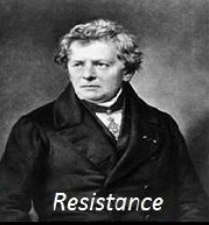
\includegraphics[width=0.5\textwidth]{../categories/media/SIunits/GeorgOhm.png}
	}
	\only<2>{
		Who is Georg Ohm?
	}
\end{textarea}
}


\def \Qd % 2
{
\begin{textarea}[]
	\only<1>{
		\centering
		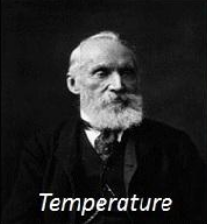
\includegraphics[width=0.5\textwidth]{../categories/media/SIunits/WilliamThomason_LordKelvin.png}
	}
	\only<2>{
		Who is William Thomason (Lord Kelvin)?
	}
\end{textarea}
}

\def \Qc % 2
{
\begin{textarea}[]
	\only<1>{
		\centering
		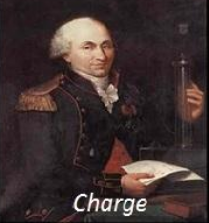
\includegraphics[width=0.5\textwidth]{../categories/media/SIunits/CharlesAugustinDeCoulomb.png}
	}
	\only<2>{
		Who is Charles Augustin de Coulomb?
	}
\end{textarea}
}

\def \Qb % 3
{
\begin{textarea}[]
	\only<1>{
		\centering
		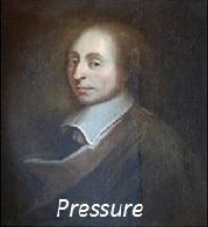
\includegraphics[width=0.5\textwidth]{../categories/media/SIunits/BlaisePascal.png}
	}
	\only<2>{
		Who is Blaise Pascal?
	}
\end{textarea}
}

\def \Qe % 4
{
\begin{textarea}[]
	\only<1>{
		\centering
		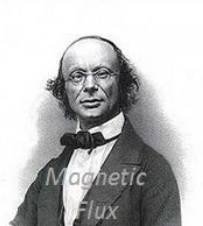
\includegraphics[width=0.4\textwidth]{../categories/media/SIunits/WilhelmWeber.png}
	}
	\only<2>{
		Who is Wilhelm Weber?
	}
\end{textarea}
}
